%--------------------------------------------------------------------------------------------------
\section{Image Recognition Models}
\label{rel:sec_imrecon}
Image recognition is a substask of computer science that aims at replicating human vision capabilities 
with a machine. Arguably, it is with the improvement and interaction of the three fundamental tasks 
of computer vision (Recognition, Reconstruction and Reorganization) \autocite{malik2016three} that we 
find this field moves forward. Interestingly, improvements in one these fundamental Rs can be 
used to drive forth its peers; moreover, (words).




%1960s, first thesis, image processing, pattern recognition
%1970s foundational work on image recognition
%1980 vision applied to maths, geometry, control theory, optimization
%1990s geometric analysis coplete, graphics,statistical learning
%200s advances in visual recognition, practical applications

Ultimately, it was with inspiration on studies on neuroscience \autocite{hubel1959receptive} that the 
development of \glspl{nn} started. In particular, the Neocognitron \autocite{fukushima1975cognitron} 
proposes the first \gls{nn} where kernel operations and feature aggregation in a hierarchical 
manner and non-linearities stand out as these contributions can be seen as the main components of a 
most recent image recogniton models.
Still, the Neocognitron's hierarchical properties and aggregation didn't really achieve 
a great deal of momentum on early days; around this time, other image recognition models were being 
used yielding better results, examples of this can be seen with the amount of traditional machine 
learning based methods that dominated this task around that time. Nevertheless, getting close to the 
dawn of the year 2000, Yann LeCun proposed LeNet to perform digit recognition 
\autocite{lecun1998gradient} the first \gls{cnn}.\\

\subsection{Convolutional Neural Networks}
\label{rel:sub_cnn}
Starting with LeNet, the convolution took prominence as the fundamental building block 
of most current image recognition models. On itself, a convolutional layer operates by the 
interaction of a kernel with a set of features. This interaction depends in 
direct correlation with the kernel size, mediated by its width and height. Furthermore, 
these kernels are meant to project features into different spaces; with this in mind we point out 
that convolutions are mostly a local operation. 
%Figure \ref{fig:conv_local} illustrates these 
%properties of the convolution operation.
%\begin{figure}[h]
    \centering
    \includegraphics[width=\textwidth]{fig/rel/images/conv_not_proper.png}
    \caption{Illustration of the convolution operation. Properties, parameters and behaviour.}
    \label{fig:conv_local}
\end{figure}

\noindent On top of convolutions, LeNet led to the introduction of more components of \glspl{cnn}: 
pooling operations and non-linearities. Pooling operations are used to reduce the spatial 
resolution of feature maps, which in turn aids convolutions in capturing features from longer 
range dependencies within the image. Moreover, via pooling it is possible to capture the most 
relevant features within a neighborhood.\\
On another hand non-linearities such as Sigmoid and ReLU, are designed to capture complex 
relationships within data, stopping the model collapsing into a linear operation. Moreover, these 
operations also contribute with stability: they maintain values within feature maps and the gradient 
in ranges in which the network can operate with. %cite this?
Still, the key contribution leading to the success of LeNet was not only the usage of 
convolutions, pooling and nonlinearities; but its training process, that guided by gradient descent 
to optimize ultimately enabled \glspl{cnn} to outperform traditional computer vision methods for 
document recognition. 

\begin{figure}[h]
    \centering
    \includegraphics[width=\textwidth]{fig/rel/images/CNN_timeline.pdf}
    \caption{Timeline of \glspl{cnn} development alongside milestone models.}
    \label{fig:cnn_timeline}
\end{figure}

\noindent With the advent of the 2010s and the initiation of the \gls{ilsvrc} \autocite{ILSVRC15} 
a proper environment for further devolpement of models was established. Unlike prior datasets, 
ImageNet was composed of images that presented more complexity than earlier datasets. Instead 
of catalogue-like compositions, for instance, elements in this dataset closely resemble those found 
in the wild, featuring multiple classes or instances of a class in a single image.

Upon its release, several traditional approaches were trained and evaluated on this collection, 
achieving a low performance. However, \glspl{cnn} regained prominence with the introduction of
AlexNet \autocite{krizhevsky2012imagenet}. Inspired by LeNet, Krizhevsky designed a 
\gls{cnn} that incorporated additional convolutions and, more importantly, facilitated faster 
computation through effective communication with the \gls{gpu}.
AlexNet gained notoriety by emerging as the winner of the 2012 \gls{ilsvrc}, achieving a top-1 
classification accuracy difference of nearly 10\% compared to previous year's winners 
(\cite{berg2010large}, \cite{sanchez2011high}). This substantial improvement in recognition 
capabilities led in a paradigm shift in various machine learning tasks, laying the foundation 
for the deep learning revolution.\\

\noindent Following this success, several \glspl{cnn} were introduced in the decade of 2010, where 
a considerable of models where introduced. Nevertheless, we can stablish a timeline with the 
milestone models that influenced the most this development, as seen in \autoref{fig:cnn_timeline}.
In the year following AlexNet's publication, an updated form of mapping feature maps into 
classification embeddings was proposed  in the shape of \gls{gap} \autocite{lin2013network}. 
This pooling protocol improves classification as it enforces correspondences between feature maps 
and categories; conversely it doesn't require any optimization whatsoever, negating effects of 
overfitting. 

\begin{figure}[t]
    \centering
    \scriptsize
    \begin{tabular}{cc}
        \mc{2}{\begin{tikzpicture}[
        font={\footnotesize},
        trap/.style={trapezium, rotate=-90,trapezium angle=75},
    ]
        %% CNN branch
        \node(input) at (0, 0) {\includegraphics[width=.1\textwidth]{fig/castream/images/input.jpg}};
        \node[above] at (input.north) {Input image $\vx$};
        \node[draw, rotate=90, align=center](conv1) at (2, 0) {\Th{conv} $7\times7$};
        %\node[draw, rotate=90, align=center](bn) at (-3, 0) {\Th{BatchNorm}};
        %\node[draw, rotate=90, align=center](relu) at (-2.5, 0) {\Th{ReLU}};
        %\node[draw, rotate=90, align=center](maxp) at (-2, 0) {\Th{MaxPool}};
        \node[draw, trap] (res1) at (4,0) {\rotatebox{90}{\parbox{1.0cm}{\centering{\Th{Res-1}}}}};
        \node[draw, trap] (res2) at (6,0) {\rotatebox{90}{\parbox{1.0cm}{\centering{\Th{Res-2}}}}};
        \node[draw, trap] (res3) at (8,0) {\rotatebox{90}{\parbox{1.0cm}{\centering{\Th{Res-3}}}}};
        \node[draw, trap] (res4) at (10,0) {\rotatebox{90}{\parbox{1.0cm}{\centering{\Th{Res-4}}}}};
        %\node[](empt1) at (6.25, 0){};
        \node[draw, rotate=90, align=center] (class) at (12,0) {Classifier};
        \node(logit) at (13, 0) {$\vy$};
    
        %% CNN backbone
        %\node(empt0) at (-4.65, 0) {};
        \draw[->] (input.east) -- node {} (conv1);
        \draw[->] (conv1.south) -- node[above] {$F_0$} (res1);
        %\draw[->] (empt0.center) -- node {} (conv1);
        \draw[->] (res1) -- node[above] {$F_1$} (res2);
        \draw[->] (res2) -- node[above] {$F_2$} (res3);
        \draw[->] (res3) -- node[above] {$F_3$} (res4);
        \draw[->] (res4) -- node [above] {} (class);
        \node[](GAP) at (11.125,0.25) {\gls{gap}};
        \draw[->] (class) -- node {} (logit);
\end{tikzpicture}
    }\\
        \mc{2}{$a.$ ResNet Architecture}\\
        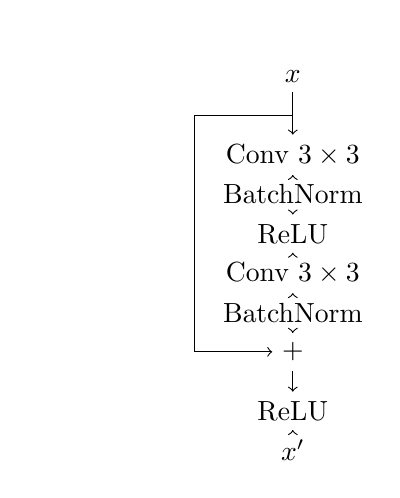
\begin{tikzpicture}[]
    % Nodes
    \node at (1.75,0) (input){$x$};
    \node[align=center] (conv1) at (1.75, -1) {\Th{Conv} $3\times3$};
    \node[align=center] (bn1) at (1.75, -1.5) {\Th{BatchNorm}};
    \node[align=center] (relu1) at (1.75, -2.0) {\Th{ReLU}};
    \node[align=center] (conv2) at (1.75, -2.5) {\Th{Conv} $3\times3$};
    \node[align=center] (bn2) at (1.75, -3) {\Th{BatchNorm}};
    \node[align=center] (sum) at (1.75, -3.5) {$+$};
    \node[align=center] (relu2) at (1.75, -4.25) {\Th{ReLU}};
    \node(output) at (1.75, -4.75) {$x'$};
    \node at (1.75,-0.5) (empt0) {};
    \node at (0.5, -2.5) (empt1) {};
    \node at (-1.5, 0.5) (emptkek) {};  

    %% CNN Edges
    \draw[->] (input.south) -- node {} (conv1);
    \draw[->] (conv1.south) -- node  {} (bn1.north);
    \draw[->] (bn1.south) -- node  {} (relu1.north);
    \draw[->] (relu1.south) -- node  {} (conv2.north);
    \draw[->] (conv2.south) -- node  {} (bn2.north);
    \draw[->] (bn2.south) -- node  {} (sum.north); 
    \draw[-] (empt0.center) -| node {} (empt1.center);
    \draw[->] (empt1.center) |- node {} (sum.west);
    \draw[->] (sum.south) -- node  {} (relu2.north);
    \draw[->] (relu2.south) -- node  {} (output.north);
\end{tikzpicture}
&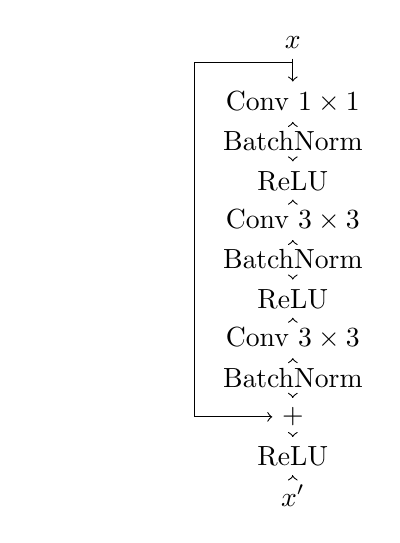
\begin{tikzpicture}[]
    % Nodes
    \node at (1.75,0.25) (input){$x$};
    \node[align=center] (conv1) at (1.75, -0.5) {\Th{Conv} $1\times1$};
    \node[align=center] (bn1) at (1.75, -1) {\Th{BatchNorm}};
    \node[align=center] (relu1) at (1.75, -1.5) {\Th{ReLU}};

    \node[align=center] (conv2) at (1.75, -2) {\Th{Conv} $3\times3$};
    \node[align=center] (bn2) at (1.75, -2.5) {\Th{BatchNorm}};
    \node[align=center] (relu2) at (1.75, -3.0) {\Th{ReLU}};

    \node[align=center] (conv3) at (1.75, -3.5) {\Th{Conv} $3\times3$};
    \node[align=center] (bn3) at (1.75, -4) {\Th{BatchNorm}};
    \node[align=center] (sum) at (1.75, -4.5) {$+$};

    \node[align=center] (relu3) at (1.75, -5) {\Th{ReLU}};
    \node(output) at (1.75, -5.5) {$x'$};
    \node at (1.75,-0) (empt0) {};
    \node at (0.5, -2.75) (empt1) {};
    \node at (-1.5, 0) (emptkek) {};
    

    %% CNN Edges
    \draw[->] (input.south) -- node {} (conv1);
    \draw[->] (conv1.south) -- node  {} (bn1.north);
    \draw[->] (bn1.south) -- node  {} (relu1.north);
    \draw[->] (relu1.south) -- node  {} (conv2.north);

    \draw[->] (conv2.south) -- node  {} (bn2.north);
    \draw[->] (bn2.south) -- node  {} (relu2.north); 
    \draw[->] (relu2.south) -- node  {} (conv3.north);

    \draw[->] (conv3.south) -- node  {} (bn3.north);
    \draw[->] (bn3.south) -- node  {} (sum.north); 
    \draw[-] (empt0.center) -| node {} (empt1.center);
    \draw[->] (empt1.center) |- node {} (sum.west);
    \draw[->] (sum.south) -- node  {} (relu3.north);
    \draw[->] (relu3.south) -- node  {} (output.north);
\end{tikzpicture}
\\
        $b.$ Basic Block Residual Block & $c.$ Bottleneck Residual Block \\
    \end{tabular}
    \caption{Generalities of the ResNet architecture. Overall architecture and Residual Block Design.}   
    \label{fig:resnet}
\end{figure}

Similar to 2012 and 2013, 2015 saw the proposal of two milestone models: the Inception architecture 
\autocite{szegedy2015going} and VGG models \autocite{simonyan2015deep}. On one hand, the Inception 
architecture is designed to learn features in different scale. To achieve this, \emph{Inception 
Block} is introduced, where the multi-scale behaviour is captured with the incorporation of 
convolutional kernels with sizes of $5\times5$, $3\times 3$ and $1\times1$. In contrast to 
the Inception architecture, VGG models are built with a simplistic design, relying solely on 
$3\times 3$ convolutions; in turn, VGG has been shown to be an excellent feature extractor network. 
Led by the desire to increase depth of \glspl{cnn}, VGG and Inception attempted to make models 
deeper; nevertheless this was not possible because of the vanishing gradient issue. As an answer to 
this, the ResNet architecture was proposed \autocite{he2016deep}.\\


%\begin{tikzpicture}[
        font={\footnotesize},
        trap/.style={trapezium, rotate=-90,trapezium angle=75},
    ]
        %% CNN branch
        \node(input) at (0, 0) {\includegraphics[width=.1\textwidth]{fig/castream/images/input.jpg}};
        \node[above] at (input.north) {Input image $\vx$};
        \node[draw, rotate=90, align=center](conv1) at (2, 0) {\Th{conv} $7\times7$};
        %\node[draw, rotate=90, align=center](bn) at (-3, 0) {\Th{BatchNorm}};
        %\node[draw, rotate=90, align=center](relu) at (-2.5, 0) {\Th{ReLU}};
        %\node[draw, rotate=90, align=center](maxp) at (-2, 0) {\Th{MaxPool}};
        \node[draw, trap] (res1) at (4,0) {\rotatebox{90}{\parbox{1.0cm}{\centering{\Th{Res-1}}}}};
        \node[draw, trap] (res2) at (6,0) {\rotatebox{90}{\parbox{1.0cm}{\centering{\Th{Res-2}}}}};
        \node[draw, trap] (res3) at (8,0) {\rotatebox{90}{\parbox{1.0cm}{\centering{\Th{Res-3}}}}};
        \node[draw, trap] (res4) at (10,0) {\rotatebox{90}{\parbox{1.0cm}{\centering{\Th{Res-4}}}}};
        %\node[](empt1) at (6.25, 0){};
        \node[draw, rotate=90, align=center] (class) at (12,0) {Classifier};
        \node(logit) at (13, 0) {$\vy$};
    
        %% CNN backbone
        %\node(empt0) at (-4.65, 0) {};
        \draw[->] (input.east) -- node {} (conv1);
        \draw[->] (conv1.south) -- node[above] {$F_0$} (res1);
        %\draw[->] (empt0.center) -- node {} (conv1);
        \draw[->] (res1) -- node[above] {$F_1$} (res2);
        \draw[->] (res2) -- node[above] {$F_2$} (res3);
        \draw[->] (res3) -- node[above] {$F_3$} (res4);
        \draw[->] (res4) -- node [above] {} (class);
        \node[](GAP) at (11.125,0.25) {\gls{gap}};
        \draw[->] (class) -- node {} (logit);
\end{tikzpicture}
    
\noindent The ResNet architecture is designed with the idea of residual connections as their 
building block. On itself, a residual generates outputs via the summation of its input and a 
linear mapping of it. This in turn enhances the network capabilities to scale in size, leading to 
improvements in performance while being easier to optimize. A thorough representation of this 
architecture is presented in \autoref{fig:resnet}. 
This architecture has maintained its relevancy because of its modularity and the aforementioned 
scaling properties. For instance, some of the most important \gls{cnn} based object detectors are 
designed using ResNet as backbone (\cite{ren2015faster}, \cite{lin2017focal}, \cite{he2017mask}). 

In a similar fashion to the residual connections introduced in ResNet, DenseNet 
\autocite{huang2017densely} was proposed with the idea of connecting all layers operating within 
matching feature-map sizes. This architecture on one hand enables the training of very deep 
models; the dense connections allow for feature reuse and identity mappings, thus negating the 
effect of vanishing gradients. However one issue that be brought forth with DenseNet is modularity 
and ease of use. Since a great number of neurons are interconnected by design, introduction of 
modifications such as \gls{nlb}\cite{wang2018non} can seem  rather challenging; whereas in 
architectures such as ResNet, this procedure is rather simple.



ResNet \cite{he2016deep}, 
Inception (\cite{szegedy2015going}, \cite{szegedy2016rethinking}), NasNet (\cite{zoph2018learning})
DenseNet \autocite{huang2017densely} EfficientNet(\cite{tan2019efficientnet}) 
ResNet Strikes back (\cite{wightman2021resnet}) \autocite{liu2022convnet}
%\addcontentsline{toc}{subsection}{Convolutional Neural Networks}

\subsection{Attention-Based Architectures}
\label{rel:sub_att}
%\addcontentsline{toc}{subsection}{Attention-Based Architectures}
Attention is a powerful mechanism that has been introduced into convolutional networks in several 
ocasions (\cite{bello2019attention}, \cite{ramachandran2019stand}, \cite{shen2020global}). 
With the success of vision transformers (ViT) (\cite{dosovitskiy2020image}), fully attention-based 
architectures are now competitive with convolutional networks. To benefit from both self-attention 
and convolutional layers, some hybrid architectures employ convolutional layers before the vision transformer 
. Others, such as Swin (\cite{liu2021swin}) and PiT 
(\cite{heo2021rethinking}), introduces a pyramid structure to share local spatial information 
while reducing the spatial resolution, as in convolutional networks. 

SCOUTER (\cite{li2021scouter}) uses slot attention (\cite{locatello2020object}) to build a class 
specific pooling mechanism, which does not scale well to more than 20 classes. 

\subsection{Hybrid Architectures}
\label{rel:sub_hybrid}
(\cite{graham2021levit}, \cite{xiao2021early})
Conformer (\cite{peng2021conformer}) proposes a dual network structure to retrain and fuse local 
convolutional features with global representations. Our method merely provides a simple 
attention-based pooling mechanism inspired by transformers that can work with any architecture, 
even pretrained and frozen. PatchConvNet (\cite{touvron2021augmenting}) replaces global average pooling by an 
attention-based pooling layer.
